

\section{Tutorial}


This section will lead you through a first exemplary run of cosmouline. Explanations for the first steps are very detailed at the beginning, but as you will see, once you know how to measure the seeing of the images you can already guess how to construct a PSF.
So don't worry and read on. Details and mechanisms are shown along the way, and it gets much faster after the first steps.


\subsection{Preparing the directories and data}

Step number 0 is to get the images ready. Let's assume you have some images somewhere on your disk. All we need is a plain directory containing FITS files. If not, you can use the two Mercator sample images I've put on the web. This directory could also be your image database: cosmouline will not modify anything in there, but it will simply copy them as soon as a first copy is required (more precisely:for the sky subtraction).


Two remarks on these images :

\begin{itemize}

\item Input images should be prereduced, and have clean borders\footnote{So if you have ``black'', ``white'', ``messy'', or ``NaN'' frames around your images, your are kindly asked to crop them \emph{before} starting cosmouline.}.
Note that there is absolutely no need to have images with homogeneous dimensions. Aside of this, the pipeline does of course \smiley\, also handle images with different pixel scales, but this is discussed later. For now start with images from one single telescope, i.e. with one fixed pixel size.

\item Cosmouline will align the images, taking into account a shift and an arbitrary rotation, with respect to a reference images we will choose later. But flips (i.e. mirror inversion) are not compensated. If your images are flipped (Mercator...), then it's now your last chance to put them back into the natural orientation before starting the pipeline.

\end{itemize}

To crop or flip your images if needed, you might look at some scripts provided in \\ \verb+0_preparation_scripts+. These are not really part of cosmouline, you will have to edit them to make them work.

Now that the images are ready somewhere on your disk, we need to prepare the 3 directories presented in the introduction :

\begin{itemize}

\item \verb+pipedir+:decompress the cosmouline tarball (as you probably already did), and here you are.

\item \verb+configdir+:start from the sampleconfig dir, by copying \verb+pipedir/sampleconfig/+ beside (and not \emph{in}) the \verb+configdir+ (for example). The files in this sample-\verb+configdir+ will all be discussed later.

\item \verb+workdir+:just make an empty directory somewhere (for instance next to \verb+pipedir+ and \verb+configdir+).

\end{itemize}

It is very useful to open a shell (or desktop) in each of these directories.

\subsection{Adjusting the central configuration file}

\tbrem{Copy sampleconfig.py into config.py (to escape from version control), use ``cp sampleconfig.py config.py'' (and not svn copy ...)}
\tbrem{Export (instead of checkout) the sampleconfig dir}

The behaviour of most of the scripts is controlled by the python file called \verb+config.py+ in your \verb+pipedir+. Open it in your favourite editor (and just keep it open). We will now have to make some changes in this file.

\begin{itemize}
 \item The first line tells the scripts on which computer they are running. Your computer is probably unknown for now, so give him a nice name.
\item Fill out the correct paths to your \verb+pipedir+ and \verb+configdir+.
\item Once this is done, provide or check the path to SExtractor under Computer Setup. 
\end{itemize}

%If you do not use the old MCS programs (in fact from the old programs, only the two psf construction programs may be used in \verb+cosmouline_1.0+ -- we will always use the latest deconvolution program), you don't have to fill those lines out.

You can mail your \verb+config.py+ to the customer support service at any time, and they will add it to the next releases of cosmouline. That's it for now, we will come back to this \verb+config.py+ later.

Next step is to fill out the other important file: the \verb+settings.py+ file in your \verb+configdir+. This file contains all the input info for the different scripts of the pipeline. At this stage you only have to specify the path to your \verb+workdir+. We will come back to this file every time a script asks for new settings.


\subsection{Meet the pipeline structure}

Move to \verb+pipedir+. In there, the ``sequencial'' pipeline scripts are grouped in numbered subdirectories, with rather explicit names starting with a number. Aside from this, there are some other directories in \verb+pipedir+:

\begin{itemize}
\item \verb+modules/+:contains python functions, modules, and classes needed by the pipeline. No need to visit this for now. But some of the pipeline code is in there.

\item \verb+extrascripts/+:some relatively userfriendly facultative scripts to interact with the process, that can be executed at different moments:that's why they are not part of the numbered scripts.

%\item \verb+docs/+:documentation of the pipeline itself and the used modules.

\item \verb+progs/+:Fortran77 programs for psf fitting, object extraction and deconvolution.

\item \verb+plotscripts/+:scripts to generate plots on the different steps. This is a rather interactive process (short scripts using matplotlib), but I will try to gather some reusable sample scripts here.

\item \verb+playground/+:not yet user-friendly experiments. The place to put new inventions.

\item \verb+sampleconfig+:example of a typical \verb+configdir+

\end{itemize}

The first numbered directory in \verb+pipedir+ is  \verb+0_preparation_scripts+. In fact, it is not really part of the pipeline, but will contain some telescope-dependent ad hoc single-usage scripts to correct messy FITS headers, flip images etc. In this run we skip this directory. For Mercator and Euler images these steps have been incorporated into the prereduction pipeline.


\subsection{Adding the images to the database and characterize them}

\subsubsection{Adding images to the database}

Before executing the first script, you will have to adapt the \verb+settings.py+ file in the \verb+configdir+.

Under the header ``import new images'' in the \verb+settings.py+ file you have to indicate a setname and a telescope name.

\begin{description}
 \item[The setname] The setname is a name that will identify a group of similar images (same telescope, same season \ldots), usually imported to the database all at once. It gets really important once you start to put images from different telescopes or CCDs into the database, or if you want to add a new season to your lightcurve, as it will allow to differentiate their treatment.

The setname is also a great way to ``parallelize'' the PSF construction. If you have 300 otherwise similar Mercator images, and you happen to have access to 3 processors, then it's a good idea to split up the images into sets of 100:``Mer1'', ``Mer2'', and ``Mer3'' for instance.

For the tutorial run, just choose any short name. As a general rule, don't use spaces or special characters in any of these names you set in the configuration files:they might be automatically used in unix filenames !

\item[The telescopename] This will trigger different ways to read the FITS-headers of the images. Choose the appropriate one from the list !
If for whatever reason you don't care about the header or you do not want to read it, choose ``NOHEADER'' as telescopename. No problem for the scripts, but all images will have mjd $ = 0.0$ etc \ldots

Further header-reading-functions will be added as soon as needed\footnote{Sure you can also tweak this yourself, it's just a few lines in the ``addtodatabase'' script. Send me your tweak !}.

\end{description}



\paragraph{Other settings}

\begin{itemize}
 \item Under the header ``switches'' check that the first switch \verb+thisisatest = False+. 
\item Under the header ``import new images'' give the path to the directory of the FITS images you want to import (all images in there will get your chosen setname and telescopename).
\item Under the header ``astrocalc'' give the correct ephemerides for your object.
\end{itemize}

% Now open the script \verb+1_addtodatabase+ itself. Check or adapt the lines corresponding to the telescopes you are using for \verb+pixsize+ (typically used to express the seeing in arcsec etc),  \verb+gain+ (e$^-$/ADU),  \verb+readnoise+\footnote{not yet used\ldots},  and the \verb+scalingfactor+ corresponding to your image set. The  \verb+scalingfactor+ is a purely relative number that is used in the alignement procedure, to identify corresponding stars on images from different telescopes. The distance between two given stars, expressed in pixels, must be proportional to this scalingfactor (i.e. smaller pixels give a higher scalingfactor). It's nothing else than the inverse value of the pixel size, but with higher precision. Only  \verb+scalingfactor+-\emph{ratios} matter, so here I've chosen to give Mercator an arbitrary value of $1.0$.

You are now ready to run the first script, so
\verb+cd+ to the \verb+pipedir+\footnote{Note that due to the execfile(``../config.py'') you always have to go (either by hand or with a script) into the subdirectories of the pipedir to start a script. You cannot do ``python 1\_character\_scripts/1\_addtodatabase.py''}, fasten your seatbelt, and

\begin{Verbatim}
cd 1_character_scripts/
python 1_addtodatabase.py
\end{Verbatim}

Usually the scripts will give you some info about what they are going to do, and how many images will be affected, before starting the task. In this case you get informed about the \verb+setname+ you have chosen, and how many FITS files were found in the directory you indicated. Then the script asks you if you want to go on. This should help you to  avoid mistakes, but it's good to know that if you are sure about what you are doing, and you don't want the scripts to ask any questions, you can change the flag \verb+askquestions = True+ in \verb+settings.py+ to \verb+askquestions = False+. In fact all the scripts use only one same question (``go on or not?''), and the answers are always just yes or no. There are no questions about choices for parameters etc. Setting \verb+askquestions = False+ is thus fully equivalent to answering ``yes'' to any question.

For now keep \verb+askquestions = True+; this way, in any script, if you made a mistake in your configuration, just answer ``no'' and the script will stop without having changed anything ! You could then correct the error and start that script again.

If everything is fine and \verb+1_addtodatabase.py+ found the number of images you expected, answer ``yes''.

The script will then start reading the headers of your images, and write some of them into a brand new database. We can now visit the \verb+workdir+, to have a first look at this database. You notice that some directories were created in this  \verb+workdir+, as well as  \verb+database.dat+, which is a plain text file, that can be read (and in principle edited) with any text editor.

\begin{Verbatim}[fontsize=\relsize{-3}]
000005|000000|recno:int|imgname:str|treatme:bool|gogogo:bool|whynot:str|testlist:bool|testcomment:str|telescopename:str|setname:str ...
1|Mer1_pb150115|True|True|na|False|na|Mercator|Mer1|/Mer1prered/pb150115.fits|1.0|0.19340976|2006-02-16|2453782.74723|53782.2472227 ...
2|Mer1_pc070405|True|True|na|False|na|Mercator|Mer1|/Mer1prered/pc070405.fits|1.0|0.19340976|2006-03-07|2453802.45363|53801.9536361 ...
3|Mer1_pc220995|True|True|na|False|na|Mercator|Mer1|/Mer1prered/pc220995.fits|1.0|0.19340976|2006-03-23|2453817.51377|53817.0137719 ...
4|Mer1_pj130432|True|True|na|False|na|Mercator|Mer1|/Mer1prered/pj130432.fits|1.0|0.19340976|2006-10-14|2454022.75194|54022.2519380 ...
5|Mer1_qb080964|True|True|na|False|na|Mercator|Mer1|/Mer1prered/qb080964.fits|1.0|0.19340976|2007-02-09|2454140.53799|54140.0379938 ...
\end{Verbatim}


For details on the database, see section \ref{kirby}, or the documentation in \verb+docs/+. In one sentence, the first line tells how many entries you have in your database and which fields they have, and then follows one line per entry. The interesting thing is that from within python, in just one line, you can select/update/etc this database using for instance convenient python dictionaries.

Most of the fields in this fresh database are quite obvious (telescopename, setname, scalingfactor, ...). One important one is called \verb+imgname+:the imgname is a string formed by concatenating the setname with the original FITS filename. It is used to identify and trace images, we want it to be unique !
Others fields require a few comments.

\paragraph{Boolean flags}

We have 3 boolean (i.e. True of False) flags for each image :

\begin{description}

\item[gogogo] is a flag to definitively demote an image, for instance because it shows a completely different field, or features a huge cosmic ray on your lens. Images with \verb+gogogo+ set to False will simply be skipped by the scripts. Do not use this flag to momentary remove an image for testing purposes ! Above that, you should not edit the database by yourself to set such a flag. Instead, as we will see later, it is much cleaner to simply write the image you want to demote into a ``kicklist'' in the \verb+configdir+, together with a brief comment on \emph{why} you want to kick it, and then let a specific script (typically in \verb+extrascripts/+) update the flags in the database. This way, all the information \emph{you} enter into the pipeline is systematically stored in \verb+configdir+, and not elsewhere.

\item[treatme] is a flag that can be set according to setnames or telescopenames (for instance), again with a script from \verb+extrascripts/+. Its purpose is to allow for instance to rebuild the PSFs for this or that set of images, or to simply add a new season to existing stuff, without treating all the images again.

As a general rule with only few exceptions, the scripts will simply run their tasks on all images that have both \verb+gogogo+ and \verb+treatme+ set to True.

\item[testlist] is a flag that allows to make some fast test runs for some scripts. Building a PSF is the best example:you would set the testlist flag to true for a few ``representative'' images, set \verb+thisisatest = True+ in the \verb+settings.py+, and the scripts run only on the selected test images. Once you are happy with the PSF, you just have to set  \verb+thisisatest = False+\ldots We will try all this later.

\end{description}

% \subsubsection{Dates}
% 
% For now, 4 fields contain info about the date and time of the exposure. Everything is given in UT.
% 
% \begin{description}
% \item[date] is a string like \verb+2006-03-07+.
% \item[jd] is a string containing the best available julian date (like \verb+2453802.45363+). Sometimes the date of the exposure is directly specified this way in the FITS header, sometimes this has to be explicitly calculated from a date and time by this first script.
% \item[mjd] is a \emph{float} containing jd $- 2400000.5$. A float is useful for sorting ! Yep, the database can directly sort while selecting images.
% 
% \item[hjd] is for now a string identical to \verb+jd+, but that should be set to the Heliocentric Julian Date in future. I still have to figure out how to do this easily. (IRAF was not reliable, it produces funny things for some headers\ldots difference between hjd and jd should make a nice wave -- easy to check that IRAF was wrong !)
% 
% \end{description}

\subsubsection{Astronomical calculations}

\begin{Verbatim}
python 2a_astrocalc.py
\end{Verbatim}

This script calculates the date and UTC time of the middle of the exposure, its modified HJD, airmass, percentage of the Moon at the moment of observing, the distance to the Moon in degrees, the altitude of the Sun and the distance to the Sun in degrees. It will warn you of ``fishy images'', taken during daytime for example...
Everything is summarized in \verb+report_astrocalc.txt+ created by the next script and which you will find in your \verb+workdir+ :

\begin{Verbatim}
python 2b_report.py
\end{Verbatim}

\subsubsection{Measuring the seeing}

Whenever possible, the scripts are split in two categories:fast ones that manipulate the database, and slower ones that just read the database once at the beginning. It then gets very easy to ``parallelize'' the slow scripts, by calling them for successive setnames one after the other (but this is essential only for the PSF construction, which otherwise tends to take some nights).

The next script is a ``slow'' one.
First open the \verb+default_see.sex+ (``see'' for seeing:this file is located in this same directory \verb+1_character_scripts+, and it's the file that will actually be used by cosmouline). You should for instance adapt the \verb+PIXEL_SCALE+\footnote{The SExtractor output is given in pixels anyway; there is no big danger if this parameter is inaccurate.} and \verb+GAIN+ to the images you want to treat, but you could also change the other parameters like the aperture or background estimation. Note that we do \emph{not} use this SExtractor run to subtract the background:it's really just to measure the seeing.

Still in the \verb+1_character_scripts+:\\
\verb+python 3a_runsex.py+\footnote{If you are using the computers at Geneva Observatory, you have to run all scripts that make use of SExtractor or Pyraf on the machines called ``obssl1'' or ``obssl2''. }


The script starts by reminding you that you should first of all adapt the SExtractor input files. As this is a very non-repetitive task that would be more complicated to automatize than to do by hand, the pipeline leaves this task to the reader. So, if you forgot to update the SExtractor input:answer \verb+no+ (the script will just stop), and open the input file mentioned above. 
Once the file is updated, run \verb+python 3a_runsex.py+ again, and this time answer \verb+yes+. One more \verb+yes+ to approve the number of images, and SExtractor will run on the original images (that get linked one after the other in this current directory), and store the resulting catalogues in \verb+workdir/ali/+.

We do not update the database here. This is the task of the next script, a ``fast'' one.
Go on with

\begin{Verbatim}
python 3b_measureseeing.py
\end{Verbatim}

This script will extract a seeing and ellipticity estimation from the SExtractor catalogues. This information will be written in the database, and thus, after the usual verification of the number of images, the script starts by making a backup copy of the database.
The following fields were added to the database :
\begin{Verbatim}
'seeing:float', 'ell:float', 'goodstars:int', 'seeingpixels:float'
\end{Verbatim}
\verb+seeing+ contains the seeing estimation\footnote{Based for now on the median of the first half of the histogram of FWHM.} in arcseconds, \verb+seeingpixels+ the same in pixels,  \verb+ell+ the ellipticity, and \verb+goodstars+ is the number of good clean stars (FLAGS $= 0$) that SExtractor found (can be seen as a measure of the depth).

Go back to the \verb+1_character_scripts+ and run
\begin{Verbatim}
python 3c_seeingreport.py 
\end{Verbatim}

This is very fast, and produces no output on the screen, but writes a report of the seeing measure into \verb+workdir/report_seeing.txt+. If the seeing could not be measured, the image will automatically be attributed default values of $-1.0$.
Open this file to get, for each setname, a table sorted by seeing and showing the results of the seeing measure :

\begin{Verbatim}[fontsize=\relsize{-2}]
      ###########       Mer1    ########

      imgname | seeingpixels |       seeing |    ell | goodstars
----------------------------------------------------------------
Mer1_qb080964 |         4.63 | 0.8954871888 |  0.059 |        79
Mer1_pc220995 |         9.72 | 1.8799428672 | 0.3265 |        77
Mer1_pc070405 |       10.505 | 2.0317695288 |  0.292 |        44
\end{Verbatim}


\paragraph{Interlude:automatic database backups \& validation script}

You can visit these backups in the \verb+workdir+, under \verb+backups/+. The filename is changed to contain the date, the time, and a keyword describing what you wanted to do \emph{before} the backup was done. So \verb+20081213_153241_seeing_database.dat+ is a copy of the database done \emph{before} it was modified by the \verb+3b_measureseeing.py+.
These backups are handy if something is wrong with the database; this can happen if a script crashes for whatever reason.

In case of doubt about the integrity of the database (because you killed a script that writes to it \ldots), it's always a good idea to restart from the latest backup (by manually copying the backup file to \verb+database.dat+). You can also ``validate'' the structure of the database (e.g. check if all field contents are coherent with their formats) by running an extrascript:

\begin{Verbatim}
cd ../extrascripts/
python validate_database.py
\end{Verbatim}
which should detect any problem. Such extrascripts can be run at any time, and they are all rather safe to call without inspecting the code \ldots
While we are at it, run \verb+list_fields.py+ to display what we have in the database. New fields are always added on top of the list, but ``recno'', the internal unique record number used by the database, is always first.

%\subsubsection{Back to the seeing measure}

\paragraph{Selecting the reference image}

It's now time to choose a good reference image for the alignment. Among the first images of the report\footnote{You might also discover some truly bad images, or images with awful seeing, no stars. The ``image-removal-policy'' of cosmouline is to keep every image as long as possible -- so don't worry about them now, we will kick them in due time.}, find one with good seeing and low ellipticity, and check the raw FITS image to be sure the image has no other problems (no cosmic on the lens and the most important stars etc). Also pay attention to the field of view of your reference image: images will be aligned and cropped to match this field of view, so avoid choosing an inherently misaligned image or you might loose useful stars.

Once you have found a suitable reference image, fill out \verb+configdir/settings.py+:
enter the name of the reference image (as shown in column ``imgname'' of the report), and its $x$ and $y$ dimensions. For later statistics also specify the coordinates of a very small region around the lens, as well as of an empty region ($100 \times 100$ pixels should be enough \ldots) to measure the standard deviation of the sky. The notation for these regions is the same as in IRAF of f2n:\verb+[xmin,xmax:ymin,ymax]+.

Save the file. If you want to see a histogram of the seeings of your image (for each setname, but for now you only have one), go to the \verb+pipedir/plotscripts+ and try \\
\verb+python multi_seeing_histo.py+.


\subsubsection{Sky Statistics}

This script calculates the level and the standard deviation of the sky. If you first want to see how this is done, you can set the switch \verb+checkplot = True+ in the \verb+settings.py+. This is normally done in combination with the testlist mechanism.

\paragraph{Interlude: the ``testlist'' mechanism}

In the \verb+configdir+, create or open \verb+testlist.txt+ and write down for instance a few representative imgnames like here:

\begin{Verbatim}[fontsize=\relsize{-2}]
Mer1_qb080964	reference image
Mer1_pb150115	small triangle
Mer1_pj130432	seeing 1.8
\end{Verbatim}

All the words following each imgname are treated as a comment. Always put the reference image in the list. As for the star catalogue files, such image lists allow the use of blank lines, and comment-lines starting with \verb+#+.

Go to the \verb+extrascripts+, and launch \verb+set_testlist.py+. This will read the \verb+testlist.txt+ you just wrote, and add a flag as well as the comments into the database. You can, at any time, \verb+inspect_testlist.py+ to get the current status from the database, and \verb+reset_testlist.py+ to erase all these flags and comments, for instance if you want to change your choice of test images.

If you now set \verb+thisisatest = True+ in the \verb+configdir+'s \verb+settings.py+, all scripts supporting the testlist mechanism (png creation, PSF construction, deconvolution \ldots) will only run on your test images. Just put  \verb+thisisatest = False+ to get back in the normal mode; nice, you don't have to to remove the testflags from the database.

\paragraph{Back to the sky statistics}

So now you can test this script on a small number of images. It will draw a plot per image. You continue with the next image by closing the previous plot.

\begin{Verbatim}
python 4a_skystats.py 
\end{Verbatim}
Once you are familiar with these plots, you can go back to \verb+settings.py+ and reset both switches, \verb+checkplot+ and \verb+thisisatest+ to False. Rerun the script and it will calculate the sky level on all images without plotting, which takes some time. The next script, a very quick one, then writes a \verb+report_skylevel.txt+ into your \verb+workdir+.

\begin{Verbatim}
python 4b_report.py 
\end{Verbatim}




\subsection{Sky-subtraction}

\begin{Verbatim}
cd ../2_skysub_scripts/
python 1_skysub.py
\end{Verbatim}

As for the previous SExtractor run, make sure that the parameters in \verb+default_sky.sex+ are adequate for your images.

This is the first script that makes an actual real ``copy'' (sky-subtracted) of the images into the workdir, under \verb+ali/+. From now on, the scripts are fully independent from the initial files specified in \verb+settings.py+; all we need is \verb+pipedir+, \verb+configdir+, and \verb+workdir+.


\subsection{Image alignment}

The image alignment is done by automatically identifying corresponding stars in the SExtractor catalogues (fast), then calling the standard IRAF tasks geomap and gregister (slow). This works for arbitrary shifts or rotations.

Before this, we have to select some stars suitable for calculating the transformation. Print out or make a sketch of the reference image, select some good stars (non-saturated, single, well-distributed around the lens, healthy \ldots), give them names (``Donald'', ``Edwin'', or just ``a'', ``b'', etc if you don't feel like joking (anyway don't use ``Mr. Bean'': no white space please !)), measure their approximate positions (in the reference image of course) using something like \verb+imexa a+, and fill out the \verb+configdir/alistars.cat+, like this\footnote{You could give the fluxes in an optional fourth column, but they would get replaced by the SExtractor fluxes very soon, not to mention that the matching algorithm does not use fluxes for now.} (but with more stars):

\begin{Verbatim}[fontsize=\relsize{-2}]
#name  xpos       ypos
a      1436.79    887.07
b       675.41    878.89
\end{Verbatim}

Note that the pipeline (and SExtractor) always uses ``image'' coordinates, and not ``physical'' coordinates or other funny fields of the ds9 window ! These image coordinates are simple counting pixels: $(0,0)$ should be on the bottom left of the frame displayed in ds9.
You can leave white lines, and use \verb+#+ as first character to comment a line. 

\begin{Verbatim}
cd ../3_align_scripts/
python 1a_checkalistars.py
\end{Verbatim}
This script reads your \verb+alistars.cat+, creates a png image of the reference image, draws circles around your reference stars, and rectangles around the lensregion and the empty region specified in \verb+settings.py+. The file \verb+alistars.png+ is stored in your \verb+workdir+ and will be very helpful throughout the pipeline.

\begin{Verbatim}
python 1b_identcoord.py
\end{Verbatim}
and you would soon see if you made an error in the \verb+alistars.cat+. Indeed, answer ``yes'', and the script will start by looking for your alignement stars in the SExtractor catalogue (the one we made to measure the seeing) of the reference image. If there is a problem, it will tell you which star is wrong. If everything is fine, it proceeds by identifying the alignment stars in all the images of the database, and writing the input files for the geomap task (in \verb+workdir/ali/*.geomap+). On the fly, some new fields are added to the database; a special flag used for the alignement procedure, the number of stars that were identified, the maximum number of stars that could have been identified (i.e. the length of your \verb+alistars.cat+), and a comment about which stars were rejected and why.

Go on with :

\begin{Verbatim}
python 1c_report.py
\end{Verbatim}

The report is sorted by the number of alignment stars, it's called
\verb+report_prealiident.txt+, and you find it in your \verb+workdir+. It allows
to see how it went, detect stars that might be problematic, visit the funny
images that could not be identified, or, for the advanced user, tweak some
parameters of the identification algorithm (explained in the first lines of
\verb+1b_identcoord.py+) and rerun the identification if needed.


If some images are out of subject and thus cannot be aligned, just leave them as they are. The next scripts know how to cope with that, they will not crash.

\begin{Verbatim}
python 2a_alignimages.py
\end{Verbatim}

This will use IRAF (pyraf) for the first time. I hope everything is fine with your installation. Normally this should use the usual \verb+login.cl+ in your IRAF-directory.

\tbrem{In case of images with large shifts with respect to the reference image, you would now have large non-overlapping regions of these files set to 0.0 ADU. Small strips of zeroes are not a problem, but if these regions cover more then say a fourth of an image, sextractor will get fooled and produce a crappy catalog. Hence there is an optional script to fill these 0.0 regions with plain noise.}

\begin{Verbatim}
python 2b_report.py
\end{Verbatim}

\ldots writes the \verb+report_postali.txt+ into your \verb+workdir+. Not much more to say. Histograms of the geomaprms can also be interesting: \verb+ cd pipedir/plotscripts+:\\ \verb+python multi_geomaprms_histo.py+, as figure \ref{geomaprmshisto} shows. 

\begin{figure}[htbp]
\begin{minipage}[c]{0.5\textwidth}
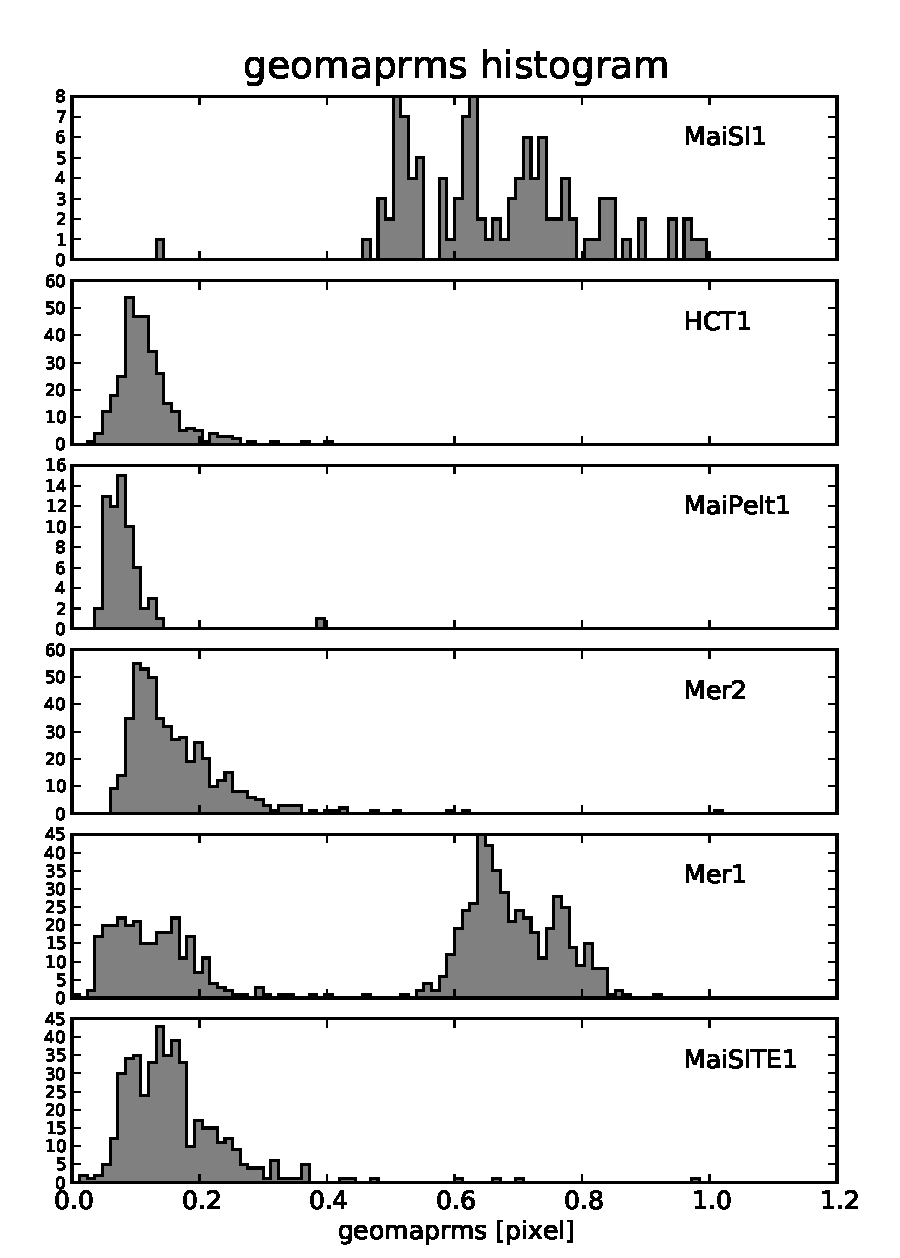
\includegraphics[width=1.0\textwidth]{images/geomaprmshisto.pdf}
\end{minipage} \hfill
\begin{minipage}[c]{.48\textwidth}
%\vspace{40pt} 
\caption{ \label{geomaprmshisto}}
%\vspace{0pt}
\captionsize{You could perhaps remove some problematic alignment stars to see if you can improve the situation for the sets ``Mer1'' and ``MaiSI1''. In the scope of this tutorial, \verb+multi_geomaprms_histo.py+ will only show one histogram, as we have only one image set for the moment.}
\end{minipage}
\end{figure}


\begin{Verbatim}
python 3_updateflags.py
\end{Verbatim}
This one updates the \verb+gogogo+ flags to \verb+False+ for all images that could not be aligned. All images remain in the database, but these will be skipped by the following scripts.

Finally, the last script will generate pngs from the aligned images, to allow a convenient systematic visual inspection. And as it is rather slow, it's an excellent occasion to do a test run on a few images before launching it on the full set. 

In the \verb+settings.py+ file, there is a switch \verb+makejpgarchives = True+. In that case, every script of the pipeline that creates pngs for inspection will ask you, once it has finished creating the pngs, if it can go on with jpg. If you answer ``yes'', it will also create jpg images and make a tarball of them so that it is easier to copy them from one computer to another. If you do not want to use this feature, either answer ``no'' or put \verb+makejpgarchives = False+.

This is the first script that uses \verb+f2n+. For optimal results, this script has to be tweaked: editing it, you can choose scales, cutoffs, cutouts, image resizing, etc \ldots That's why a little test run is useful. So setup the test run as described earlier, and launch (from \verb+3_align_scripts+)

\begin{Verbatim}
python 4_pngcheck.py
\end{Verbatim}

The result is stored in something like \verb+workdir/ali/png_full+, in form of chronologically\footnote{You can of course easily tweak all this in the script.} sorted png files. You can simply look at them with \verb+xv *.png+, which works just fine, or with any other diaporama program, like Kuickshow for example, or more sophisticated but fun, convert them to encoded movie files using for instance \url{http://ffmpeg.mplayerhq.hu/}. 
%A tarball of this entire png directory is created in the \verb+workdir+ (convenient for copies, to get those pngs on another computer for the encoding etc).


\begin{figure}[htbp]
\begin{minipage}[c]{0.5\textwidth}
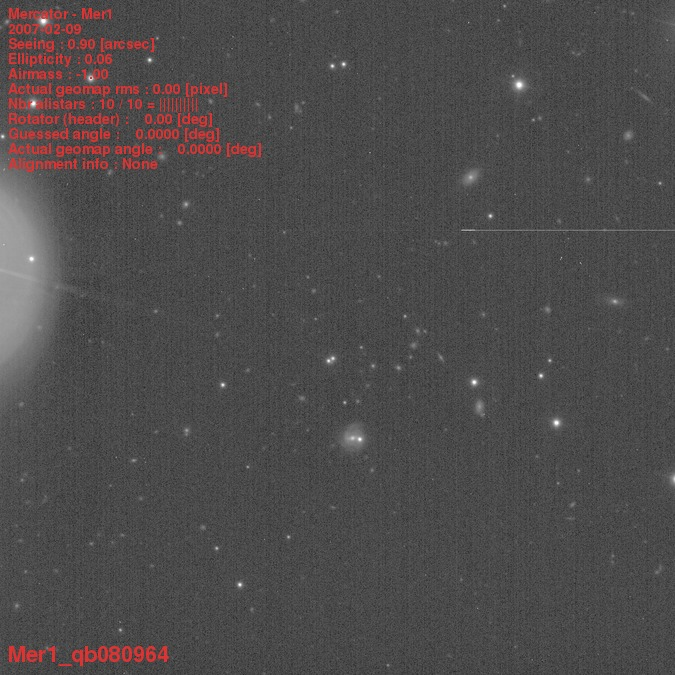
\includegraphics[width=1.0\textwidth]{images/alipng.jpg}
\end{minipage} \hfill
\begin{minipage}[c]{.48\textwidth}
%\vspace{40pt} 
\caption{ \label{alipng}}
%\vspace{0pt}
\captionsize{If everything works, your pngs should look like this. This is in fact a reference frame, hence the 0.00 angles and rms-values.}
\end{minipage}
\end{figure}


Note that by default, all these png-making scripts simply delete (after a warning) all already existing pngs (if you don't explicitly tweak the ``pngkey'' at the beginning of these scripts). You can try this for instance by setting \verb+thisisatest = False+ and rerun the script. If you want to keep your movies safe, just get them out of the \verb+workdir+. You can also delete them to free some diskspace, at any time.

Another way to free some disk space is to use the last script stored here, which is facultative:

\begin{verbatim}
 python 5_facult_removeskysub.py
\end{verbatim}
It will remove the sky-substracted images before alignment in the \verb+workdir/ali/+. You can reconstruct them at any time if you need them (not necessary for the pipeline) by going back to the sky substraction scripts.

\paragraph{Interlude:``definitively'' removing some images}
After looking at those pngs, or perhaps zoomed cutouts on the lens, you might have found images that simply cannot be used in the lightcurves. You can set the flag \verb+gogogo+ to false for those by writing their names in \verb+configdir/kicklist.txt+ in the same way as for the \verb+testlist.txt+ above, together with an optional comment, and then running \verb+python set_gogogo.py+ from the \verb+extrascripts+.

Don't remove too many images for now; you can repeat this procedure at any time later.

\subsection{Prenormalization}
Why \emph{pre}normalization ? In order to create the PSFs for every image as a next step, we need a normalization coefficient between every image and the reference image. But given the fact that MCS is a better photometric technique than SExtractor's apertures, we will \emph{re}normalize light curves after the deconvolution, using deconvolved stars instead of using the coefficient we are going to calculate now. This way of proceeding can reduce the systematic errors due to PSF problems. So this prenormalization is not that crucial, as a better normalization follows, but nevertheless necessary to allow a common background to fit all the images in the deconvolution process of some stars. The result of the operation is just one coefficient written into the database; we do no modify the images here.

All this is now a piece of cake. Fill out the \verb+normstars.cat+ in the same way as the \verb+alistars.cat+ (you could invent a new numerotation or go on with the same names as before). Good stars are close to the lens, have the same colour, and about the same flux. You can easily check the colours of stars with Google Sky for example.


\begin{Verbatim}
cd ../4_norm_scripts/
python 1_imstat.py
\end{Verbatim}
runs IRAF imstatistics on the lensregion and the empty region (defined in \verb+settings.py+) of the aligned images to estimate the noise. The statistics on the lensregion are not used for the moment.

\begin{Verbatim}
python 2_runsex.py
\end{Verbatim}
Do not forget to check the pixelsize and gain of your telescope in the \verb+default_norm.sex+. We make new photometry catalogues from the aligned images.

\begin{Verbatim}
python 3a_calccoeff.py
python 3b_report.py
\end{Verbatim}
These scripts finally compare fluxes from the images to fluxes from the reference frame and calculate a simple but quite good median-based multiplicative coefficient, which gets written into the database. The report is written to \verb+report_prenorm.txt+.


\paragraph{Stacking images}

If you want to combine some images, now that they are aligned and that we know their flux ratios, you can combine some of the best images according to some criteria you can adapt yourself in the \verb+settings.py+: choose a maximal seeing in arcseconds, a maximal ellipticity, a maximal normalization coefficient (you have just calculated) and finally a maximal sky sigma. You also have to choose a name for your combined image.

\begin{Verbatim}
python 4a_fac_prepcombi.py
\end{Verbatim}
This first script will tell you how many images it has found that satisfy your criteria, and will put the normalized images aside in a directory \verb+workdir/combi/+. You can now do

\begin{Verbatim}
python 4b_fac_combibest.py
\end{Verbatim}
which is the actual median-combination of the chosen set of images. The outcoming combined fits image will be stored in the \verb+workdir+ directly.

% \paragraph{SExtractor flux}
% 
% Two other optional scripts...
% \begin{Verbatim}
% python build_sexfluxdb.py
% python plot_sexflux.py
% \end{Verbatim}


\subsection{PSF constructions}


We come to the core. Building a good set of PSFs (i.e. one independent PSF for each image) will require some tests and some comparisions. One central feature of cosmouline is the use of a user-chosen ``psfname'' to identify such a set of PSFs. 


Let's say you want to make a PSF with two stars, named ``a'' and ``c''. First thing to do is to choose a psfname in \verb+settings.py+. If you plan to use the new PSF construction program (that's what we will do in this tutorial), you could for instance choose a name like \verb+psfname = "new_ac"+. As written in the comments, don't change the other parameters of \verb+config.py+ unless you know what you are doing.

Now go into the \verb+configdir+, and create or adapt the file \verb+psf_new_ac.cat+\footnote{The scripts are smart enough to tell you if this file does not exist, but it \emph{does} exist in the sample configdir you are using, so it's better to not forget to adapt it.} (as you guess, replace \verb+"new_ac"+ with whatever psfname you've chosen). This file is again a catalogue file, that will be read by the same function as all the other catalogue files :

\begin{Verbatim}[fontsize=\relsize{-2}]
# psf with stars a and c
a	1436.79	887.07	400000.
c	1685.80	764.17	700000.
\end{Verbatim}

Here we have added a fourth column, containing the flux of these stars, as measured on the reference image with IRAF's ``imexa a'' command. This time the hand-written catalogue is intentionally \emph{not} cross-checked with a SExtractor catalogue, so you have to give the flux. It seems a bit too manual, but it's not a big deal and this allows you to tweak the PSF centre and flux values by hand: they will be directly used as input for \verb+extract.f+\footnote{The script will adapt these fluxes for each image, using the prenormalization, before writing the input file for the psf construction.}.


Now set  \verb+thisisatest = True+, as the PSF construction is all but fast. You always have to execute all scripts from the first to the last one of this part on either the testlist or the whole stack of images. Do not change between \verb+thisisatest = True+ and \verb+thisisatest = False+ within this series of scripts.

In \verb+pipedir+, there are 3 directories starting with a ``5'', as all these 3 tasks can be performed repeatedly and in random order but the first one is the only necessary for this tutorial run:
\begin{description}
\item[5\_new\_psf\_scripts] builds a PSF with the newest f77 MCS program
\item[5\_old\_psf\_scripts] builds a PSF using the older f77 MCS programs, controlled by the simple parameters $\lambda_{\mathrm{inner}}$, $\lambda_{\mathrm{outer}}$, and $r_{\lambda}$
\item[5\_pymcs\_psf\_scripts] builds a PSF with a new Python MCS program. This is still being developped and should not be used yet.
\end{description}
We will now start with the new PSF, but the procedure for the old one would be very similar.

\begin{Verbatim}
cd 5_psf_scripts/
python 1a_extract.py
\end{Verbatim}
This first script extracts the cutout images as well as the corresponding sigma images.
Carefully, the script asks you a few questions. These questions and warnings would be different if your psfname already existed: it is well possible to rerun all these PSF creation scripts for a subset of existing PSFs under that same psfname. The full PSF construction will happen in \verb+workdir/psf_new_ac/+.

The extraction itself is quite fast. A new flag is added to the database, and for the first time in this tutorial, the field has a \emph{name} that depends on your psfname. In this case, it is called \verb+flag_psf_new_ac+. It indicates which images are available for a given psfname. The next scripts in \verb+5_psf_scripts/+ rely on this flag, as well as on the usual \verb+treatme+- and \verb+gogogo+-flags, to determine on which images they should run.

The input files used for all the fortran programs are located in your \verb+configdir+, as templates. We have just used \verb+template_extract.txt+. You can have a look at this file, it would be straightforward to change something.

\begin{Verbatim}
python 1b_replacenan.py
\end{Verbatim}
\ldots will correct output of \verb+extract.f+ for ``NaN'' pixels and similar problems.

\begin{Verbatim}
python 2a_findcosmics.py
\end{Verbatim}
This script uses \verb+cosmics.py+, which can be found in the \verb+modules/+, to locate cosmics on the g001.fits images. These cosmics are masked only in the sig001.fits and not in the images themselves. The database is updated with the number of cosmic rays found.

If you want to mask any area of your images that you do not want to be used for the psf fitting, you can create a ds9 region file. It should be stored in your \verb+configdir+ under the name \verb+psf_psfkey_mask.reg+. Then you can execute 

\begin{Verbatim}
python 2b_applyDS9mask.py
\end{Verbatim}
If not, just go on with

\begin{Verbatim}
python 2c_reportandpng.py
\end{Verbatim}
As the name says, it adds a \verb+report_cosmics_psf_new_ac.txt+ to your \verb+workdir+ as well as a directory \verb+psf_new_ac_cosmics_png+ with pngs of those images on which cosmics have been detected and masked.

\begin{Verbatim}
python 3_writeinput.py
\end{Verbatim}
This script will prepare the input file for \verb+psf.f+. Have a look at \verb+template_psfmofsour8.txt+ in your \verb+configdir+, in which you can edit all the parameters. There is a commented version of this input file, \verb+commented_psfmofsour8.txt+, provided in the \verb+sampleconfigdir+. The filled in input files per image, ready for use after you have run this script \verb+3_writeinput.py+, can be found in your \verb+workdir/imgname+.
With this template system, the advanced reader can also adapt parameters manually. If you know good parameters, share them !

\begin{Verbatim}
python 4_buildpsf.py
\end{Verbatim}
This is the slowest script of the whole pipeline. If you have different setnames in your database, you can easily tweak it to run on only one setname, launch it, change to the next setname, launch it, and so on. The script does not write to the database (in fact it only reads the database once, at the very beginning), so there is no danger of conflict.
You can also use the version \verb+multicpu_buildpsf.py+ that automatically uses up to 4 processors if available.

The advanced user can have a look at the output files of the f77 program directly. They are stored separately per image in the \verb+workdir/psf_new_ac/imgname/+. You could for example restart from the output values for the centre and the fluxes given in \verb+psfmofsour8.out+ of the reference image: copy them into your catalogue file \verb+psf_new_ac.cat+ and go back to script \verb+3_writeinput.py+. 

After the PSF creation, you can again make some quicklook pngs, with 

\begin{Verbatim}
python 5_pngcheck.py
\end{Verbatim}
Again, the png creation will by default intentionally start by erasing any previous pngs for your psfname. If you want to keep them, move the tarball out of the way, or tweak the script.

\begin{figure}[htbp]
\begin{minipage}[c]{0.6\textwidth}
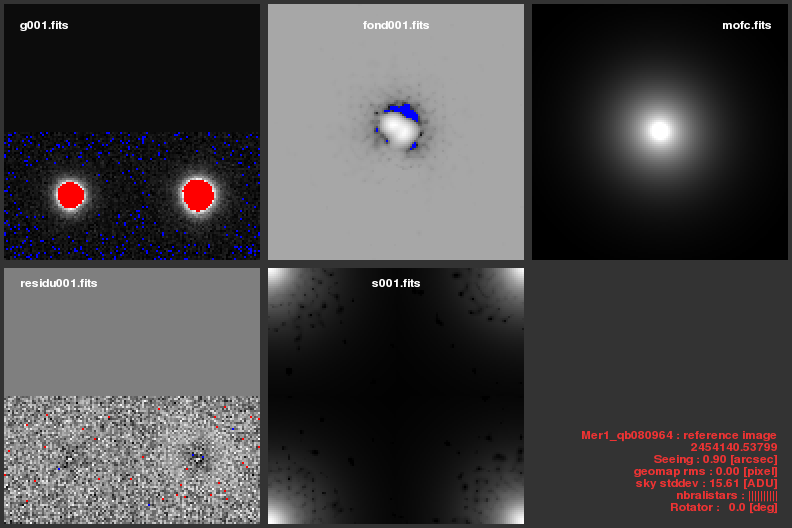
\includegraphics[width=1.0\textwidth]{images/psfpng.png}
\end{minipage} \hfill
\begin{minipage}[c]{.36\textwidth}
%\vspace{40pt} 
\caption{ \label{psfpng}}
%\vspace{0pt}
\captionsize{PSF composition. Again, cutoffs etc can be tweaked directly in the script. Even if your PSF construction started with \verb+thisisatest = False+, you can set \verb+thisisatest = True+ for the png-creation scripts to experiment with cutoffs on a small number of images, before pnging the full set.}
\end{minipage}
\end{figure}

Carefully inspect these pngs, especially the background (``fond'') and the residuals of the PSFs to see whether you have to adapt parameters or not. Once you are happy with your PSF parameters, rerun all the scripts from this directory with \verb+thisisatest = False+. Or if you want to experiment with a different smoothing, you could choose a new psfname and repeat the PSF construction.

While systematically inspecting all your PSF pngs, you will find some images for which the PSF is deformed by CCD glitches, or simply for which the residuals are too strong. Write the name of these images, as well as an optional comment (same format as for the previous image lists) in \verb+psf_new_ac_skiplist.txt+, which is a black-list for any deconvolution using this psfname. You might want to group your images by the ``kind'' or position of defaults they show (for instance, images that have cosmics on star ``a'', on star ``b'', etc). This is handy if you then want to rebuild a new PSF for a subset of your images, removing this or that star (this can be done using the testlist).

The big difference to the kicklist or the testlist is that we will \emph{not} translate these psf-skiplists into flags in the database ! The deconvolution scripts will explicitly look for these files when deciding which PSF to use with which image.

\subsection{Extracting an object for deconvolution}

While your computer is buzy calculating all the PSFs, which can take hours or even days depending on the number of images and the number of processors being used, you can already go on with the next part: extracting the small (typically 64 $\times$ 64) cutouts of the lens or some stars, for deconvolution. This process is now completely separated from the extraction of PSF stars, even if it still uses the \verb+extract.f+ program. The idea is that you can extract some objects, and then deconvolve them with different PSFs of your choice.

This has to be done for the lens and for all the stars you want to use for normalization later on. But be careful: do not execute several extractions in parallel as these scripts write things into the database! You will have to do them one per one.
Choose an objname (like ``lens'' for the lens or ``a'' for star a) in \verb+settings.py+, following the same principles as for the psfname. Fill out the corresponding catalogue file (\verb+obj_lens.cat+) with one source, like in

\begin{Verbatim}[fontsize=\relsize{-2}]
# the lens, for extraction :
lens	1002.00	955.00
\end{Verbatim}
Again: as everywhere we use ``image'' coordinates, displayed by ds9 so that the lower left corner has $(0, 0)$.

The first script will use the same \verb+template_extract.txt+ as for the PSF construction, so check the gain and pixelsize for your telescope. Again, you could use the \verb+thisisatest+ mechanism if you want to check the coordinates you put into your catalogue files, or just before the last script to check cutoffs for the pngs.

\begin{Verbatim}
cd 6_extract_scripts/
python 1a_extract_obj.py
python 1b_replacenan.py
python 2_findcosmics.py
python 3_pngcheck.py
\end{Verbatim}

All this extraction is completely unrelated to a particular set of PSFs: we will extract the lens from as many images as possible (\ldots as usual, using \verb+gogogo+ and \verb+treatme+).

If you launch the extrascript \verb+list_fields.py+, you will discover that there is now a new field in our database, called \verb+flag_obj_lens+ in this case. As for the psf construction, this boolean flag is \verb+True+ for all images from which you extracted the lens.

The pngs show you the close up on the object, again for systematic inspection. In case of a glitch or cosmic on the lens, you can't do much more than adding the image name (and the famous comment) to the \verb+kicklist.txt+, and run the extrascript \verb+set_gogogo.py+ again. It's also time now to get rid of images that are too faint or feature tracking problems etc as, at last, the next section treats the simultaneous deconvolution.

\subsection{Deconvolution(s)}

It is a good idea to first deconvolve some stars, one per one, before doing the lens deconvolution. This allows you to create first a new renormalization coefficient based on the deconvolution of various stars before coming back to the simultaneous deconvolution of your lens, in which you can then use this new renormalization coefficient instead of the previous one based on SExtractor photometry.

In practice: repeat this set of \verb+7_deconv_scripts+ on some stars, then go to the set of \verb+8a_renorm_scripts+, come back to the \verb+7_deconv_scripts+ to use them on the lens, before going to the optional \verb+8b_lookback_scripts+ and end with the final set of \verb+9_lightcurves_scripts+.

The major work of the first script is to put together the PSF and object you want for each image, respecting all the flags and kicklists, and attributing the right filenames for \verb+deconv.f+. The deconvolution supports the testlist mechanism, which should be used to look for a good set of parameters.

In \verb+settings.py+,  choose a \verb+decname+, for instance ``test1''. Specify which object you want to deconvolve by putting an existing objname in \verb+decobjname+, and write your psfname in the \verb+decpsfnames+. This is an ordered list ! You can give one single psfname, or add multiple ones, like for instance in :

\begin{Verbatim}[fontsize=\relsize{-1}]
decpsfnames = ["my_general_PSF", "better_PSF_for_some_specific_images"]
\end{Verbatim}

The psfnames in the list have increasing priority; for each image, the last one for which a PSF is available will be chosen.

Note that the deckey (the string used to identify all the stuff related to the deconvolution and defined in \verb+config.py+) also contains the chosen objname and the psfnames, so afterwards it should be rather explicit what you meant with ``test1''.

You should then specify the \verb+decnormfieldname+. When you start by deconvolving stars, you can only use \verb+medcoeff+ here. Once you will have created a new renormalization coefficient based on the deconvolution of these stars, you should put here the renormfieldname you have chosen in the next set of \verb+8a_renorm_scripts+.

\begin{Verbatim}
cd 7_deconv_scripts/
\end{Verbatim}

The first script is entirely optional but very useful for the deconvolution of the lens itself. It allows you to select images according to three quality criteria: the seeing, the ellipticity and the prenormalization coefficient medcoeff. You have to specify the maximal values for these criteria in the script itself.

\begin{Verbatim}
python 0_facult_autoskiplist.py
\end{Verbatim}

It will first show you three histograms, one for each criteria, showing in red where you situated your upper limit in the histogram. When you close these figures, it gives you a list of images that do NOT fall into the combination of your three criteria. You now just have to copy this list and paste it into the specific decskiplist of your deconvolution. These images will not be used for that deconvolution.

\begin{Verbatim}
python 1_prepfiles.py
\end{Verbatim}
Before linking all the needed FITS files into a single directory like \verb+dec_test1_lens_new_ac+ in the \verb+workdir+, it will give you a summary of the number of images that can or cannot be used. Two fields are added to the database, with customized field names: one contains the \verb+deconv.f+-prefix (0001, 0002, \ldots), the other one contains the used psfname, so that the PSF choice is traceable.


\begin{Verbatim}
python 2_applynorm.py
\end{Verbatim}
\ldots applies the prenormalization coefficients to the extracted object and sigma images.

You now have to provide the initial values for the point sources. Go to your \verb+workdir+, open the cutout from the reference image, which is called \verb+obj_lens_ref_input.fits+ for example, and estimate the initial positions and the intensities with IRAF's ``imexa x'' and ``imexa a'' for the point sources, i.e. the different lensed images in case of the lens or the single star you want to deconvolve. In the \verb+configdir+, fill in the \verb+dec_decname_decobjname_decnormfieldname_decpsfnames_ptsrc.cat+ (example: \verb+dec_test1_a_medcoeff_new_ac_ptsrc.cat+). It's again a catalogue with the objname, $x$, $y$\footnote{$x$ and $y$ in ``large'' pixels: the script will convert those values for you.}, and intensity\footnote{It can be shown that the flux measured in the input image is a good approximation of the peak value in ADU in small pixels in the deconvolved image, and that is what the program wants in fact... See demonstration in commented input files.}, like for instance :

\begin{Verbatim}[fontsize=\relsize{-2}]
# J1001
A	26.87	29.38	100000.
B	39.63	36.63	80000.
\end{Verbatim}
Bear in mind that the coordinates here are different from those used in the previous catalogues, as you are working here with the physical coordinates of the cutouts! In the catalogue for the deconvolution of the lens, the name of the QSO-images is important, as they will be used when writing the deconvolution results to the database. Try to use capital letters for these QSO images to distinguish them from the stars for which we have used small letters throughout the pipeline.

If the images of your lens are too close, then IRAF's ``imexa a'' will not give you the correct values for each of the images separately. You can then use ``imexa x'' on the central pixel, the visual peak of the image, use these coordinates and transform the given value of that pixel into a flux by using the following formula: flux = peak*seeing*seeing*1.133 with the seeing of the reference image expressed in pixels, which you can find in the \verb+report_seeing.txt+ in your \verb+workdir+.


\begin{Verbatim}
python 3_fillinfile.py
\end{Verbatim}

\ldots writes the input files for the deconvolution. Note that you can repeat the deconvolution from any of those scripts, in case you want to change the normalization, the initial flux values, positions, steps\ldots. No need to start from \verb+1_prepfiles.py+, as long as you don't change something to the PSFs.

\paragraph{Tweaking input files for the advanced user}

There are two input files for the f77 deconvolution program: \verb+deconv.txt+ and \verb+in.txt+, for which you can find templates in your \verb+configdir+ and commented versions in the \verb+sampleconfig+. These files are filled in automatically by the previous script and stored in \verb+workdir/dec_deckey/+. The previous script adapts the input of the catalogue file in two ways: the intensities are normalized per image and the coordinates for the sources to be deconvolved are transformed in small\footnote{every pixel is subdivided into four smaller pixels, which allows us to reach a higher precision in deconvolution} pixels used in the deconvolution program. 

If you want to adapt steps for coordinates of the sources, for their intensities, for the shifts between the images (delta) or for the background for all your deconvolutions, then you had better do this in the template files before executing the previous script. But if you want to change them just for one try on a specific object, then you can do it directly in the \verb+workdir/dec_deckey/+ after the previous script but before starting the deconvolution itself.
Keep in mind that these steps depend on the number of iterations the deconvolution needs before converging: if convergence is reached after 10 iterations, your steps must be 10x bigger than if convergence is only reached after 100 iterations.

There are two output files: \verb+in2.txt+, being a copy of the input file but filled in already with the output values, and \verb+out.txt+. This last one will be read by the last script in order to update the database.


\begin{Verbatim}
python 4_deconv.py
\end{Verbatim}
\ldots just launches the deconvolution. The database is not touched at all.

\begin{Verbatim}
python 5a_decpngcheck.py
\end{Verbatim}
\ldots makes pngs, as usual. It first makes a png of the reference image, so that you can check it before answering if you want all the pngs to be made or not. Typically, if you are not satisfied with the residuals or the background, you answer no, and you can go back to one of the previous scripts. 

After a first deconvolution, you might want to start again from the values towards which the first deconvolution has converged. A very helpful script for that is

\begin{Verbatim}
python 5b_showptsrc.py
\end{Verbatim}
It shows the output values for the coordinates and the intensities in a way that you can directly copy these lines into your point source catalogue file and restart from script \verb+3_fillinfile.py+.

The advanced user could also go into the \verb+workdir/dec_deckey/+ and \verb+cp in2.txt in.txt+, the file \verb+in2.txt+ being a copy of the input file but filled in already with the output values. This is particularly useful if you want to start again from output values for other parameters than coordinates and intensities, for example: delta values or values of an analytical model. In that case, do NOT use the script \verb+3_fillinfile.py+, but immediately launch the deconvolution with \verb+python 4_deconv.py+.

Once you are satisfied with the results of your deconvolution, you go on with

\begin{Verbatim}
python 6_readout.py
\end{Verbatim}

\ldots is one of the best: it reads the \verb+out.txt+, and writes its full content into the database. We add a lot of fields, with automatically generated names, also using the source names you specified in \verb+lens_ptsrc.cat+ :

\begin{Verbatim}[fontsize=\relsize{-2}]
out_dec_dec1_lens_new_ac_delta2  <type 'float'>  Shifts
out_dec_dec1_lens_new_ac_delta1  <type 'float'>  
out_dec_dec1_lens_new_ac_z2      <type 'float'>  Background parameters
out_dec_dec1_lens_new_ac_z1      <type 'float'>
out_dec_dec1_lens_new_ac_B_y     <type 'float'>  y position of image B
out_dec_dec1_lens_new_ac_B_x     <type 'float'>  x position of image B
out_dec_dec1_lens_new_ac_B_int   <type 'float'>  Intensity of image B
out_dec_dec1_lens_new_ac_A_y     <type 'float'>  y position of image A
out_dec_dec1_lens_new_ac_A_x     <type 'float'>  x position of image A
out_dec_dec1_lens_new_ac_A_int   <type 'float'>  Intensity of image A
decfilenum_dec_dec1_lens_new_ac  <type 'str'>    0001, 0002, ...
decpsf_dec_dec1_lens_new_ac      <type 'str'>    psfname used for this image
\end{Verbatim}

After a few deconvolution tries, the database could get massive and cluttered. So it is a good idea not to use this script after every test, only when you do a deconvolution, with which you are satisfied, and on all images. If you come to the conclusion that you do not need a certain try, then you can ``remove'' a deconvolution by erasing the corresponding directory in \verb+workdir+, and by removing all related fields (i.e. those shown above) from the database. To remove any field, use the extrascript \verb+remove_fields.py+: launch it, and you can enter a substring of fieldnames (like \verb+dec_dec1_lens_new_ac+) to batch-remove them.

Finally, to draw lightcurves and compare or renormalize deconvolutions, all we will need is this database.  


\subsection{Renormalization}

\begin{Verbatim}
cd 8a_renorm_scripts.py
\end{Verbatim}

These scripts allow you to determine a new and better renormalization coefficient using deconvolved sources on an image-by-image basis, which will be added to the database.

In \verb+settings.py+ you first have to choose a \verb+renormname+. It's easier for you if this name reflects the stars you are using for this renormalization, for example ``abce1''. Then under \verb+renormsources+ you should make a list of all the sources you want to include in this renormalization. For each source, you have to give the \verb+deckey+, built up as follows 

\verb+dec_decname_decobjname_decnormfieldname_decpsfnames+, and the \verb+sourcename+, for example: `dec\_test1\_a\_medcoeff\_ac1', `a' if you want to use the fluxes for star ``a'' obtained through the deconvolution run ``test1'' in which you have deconvolved star ``a'' with ``medcoeff'' as the prenormalization coefficient and the set of PSFs fitted on stars ``a'' and ``c''.

\begin{Verbatim}
python 1a_renormalize.py
\end{Verbatim}
Before adding these new coefficients to the database, you can inspect a graph that plots the individual coefficients per image and per star against time. You should check the stability of these coefficients: maybe, one star's coefficient is systematically higher/lower than the others. In that case you should not use it. When closing this first plot, a next one pops up, showing the new median coefficient per image and the old medcoeff. If both plots seem OK to you, just close it again and the median coefficient per image will be written into the database. 

Just for your background information: how are these new coefficients calculated?
We first divide the intensities of your chosen stars by the old ``medcoeff'' so that we start in a ``clean'' way. Then for every star, we calculate its median intensity over all images. Next, for every image the star's intensity is divided by this median value. We now have an intensity ratio per star and per image. In order to group these ratios together by image, we take the median value of the star intensity ratios of the same image. They already are normalization coefficients per image, but as a last step, they are rescaled in a way that the reference image takes a renormalization coefficient of 1.

\begin{Verbatim}
python 1b_report.py
\end{Verbatim}
writes a \verb+report_renorm_renormname.txt+ into your \verb+workdir+ as usual.

As explained before, go back now to the deconvolution of the lens with these new renormalization coefficients before going on with the summary of your work.

\subsection{Looking back on your work}

\begin{Verbatim}
cd 8b_lookback_scripts.py
\end{Verbatim}
This is an extremely useful tool to summarize and evaluate your work. Go to the \verb+settings.py+ file and indicate under the deconvolution header for which deconvolution you want to make this summary, usually for a complete deconvolution of the lens with a renormalization coefficient based on the deconvolution of stars. 

\begin{Verbatim}
cd 1_buildpages.py
\end{Verbatim}
asks you first to verify what you want to do and then creates the page for the reference image. Check if the scale on the right plot is okay, if not you answer no and change the scale in the \verb+settings.py+. 

The left-hand plot shows you the whole lightcurve but without grouping the points per night. The red points indicate where you are. The right-hand plots are zooms on this lightcurve, one with a variable scale, and the second one, reached by skimming, with a fixed scale.

The images underneath correspond to this red point of the lightcurve. On the left you see the extracted lens, and when skimming on this image, you get the residuals of the deconvolution. The right-hand image shows the extracted stars used to build the PSF. Skimming shows you the residuals of the PSF fitting and the background added to the Moffat function (the PSF consisting of this Moffat function plus a numerical background).

You can now navigate through the lightcurve by clicking on the bar on top: go forward or back by 1, 5, 50, or even 200 points and check whether deviating points are due to an image with a bad seeing, a badly fitted PSF or to any other of the parameters available. You can now decide to redo any part of this pipeline, or go on with plotting lightcurves. 

\subsection{Plotting and exporting lightcurves}

Finally. The open end.

Once you have deconvolved some stars and the lens with a few PSF variants, all at once or in groups by setnames etc, the database gives lots of ideas for plots. There is not a real order in which you have to execute these scripts, they are just sorted by complexity but you can pick out the one that suits you best. Here is a description of the  possibilities.

\begin{Verbatim}
cd 9_lightcurves_scripts
python 0_mag_hjd.py
\end{Verbatim}

This is a very first plot of the deconvolution results for which you indicate the name in \verb+settings.py+. For every source, it transforms the resulting flux into (relative) magnitudes and plots them as a function of time. A different colour is assigned per source. Images are not combined per night, and there are no error bars.

\begin{Verbatim}
python 1a_nightstats.py
\end{Verbatim}

Before combining the images per night for the deconvolution mentioned in \verb+settings.py+, this script just gives you some statistics on these combinations: for a given number of images per night, it tells you how many nights there are with this number of images.

\begin{Verbatim}
python 1b_firstlc_byqsoimage.py
\end{Verbatim}

Again for the same deconvolution, this plot shows the light curve of relative magnitudes against time for images grouped per night with error bars. The plotted magnitudes are the median value per night and the error bars are nothing more than the spread, the most extreme, of these values, so they are most probably asymmetric. If there is only one image per night, it does not have an error bar, which is of course not logical. Colours represent sources.

\begin{Verbatim}
python 1c_firstlc_bysetname.py
\end{Verbatim}

This is a very similar plot to the previous one, except that it uses a different colour for each set and not for every source. As you would typically use a new setname for another telescope, you can easily check systematics between telescopes.

\begin{Verbatim}
python 2_compare_decs.py
\end{Verbatim}

Before using this script, you should edit it and specify which deconvolutions you want to plot and for which source. You can compare different deconvolutions of the lens for the same source or compare the deconvolutions of stars or combine both. Magnitudes are per image and not per night, and there are no error bars so that the difference between deconvolutions per image becomes visible. Every deconvolution has its own colour. You can specify an optional magnitude shift in case your curves overlap.

\begin{Verbatim}
python 3_separate_by_telescope.py
\end{Verbatim}

Again you have to edit this script and indicate which deconvolutions you want to compare. This should typically be used for a same source observed on different telescopes. Contrary to the previous script, images are grouped by night here. Of course, every telescope has its own colour.

\begin{Verbatim}
python 4a_seeingscatter.py
\end{Verbatim}

Also here you have to tell the script which deconvolutions you want to plot. On top of plotting the lightcurve grouped per night, this script uses a colour scale to indicate the mean seeing per night for every point of the light curve, which allows you to check very quickly if deviating points are due to a bad seeing.

\begin{Verbatim}
python 4b_otherscatter.py
\end{Verbatim}

The previous script is in fact just an example how you can colour-code other parameters on top the lightcurve. The only difference with this one is line 54: instead of the mean of the seeing, we take the mean airmass, but why not try a median value or ellipticity or \ldots Do no forget to adapt the minimum and maximum value for your colour scale on line 64.

\begin{Verbatim}
python 5a_calc_indiv_errors.py
\end{Verbatim}

The next two scripts are a first try to calculate error bars on the individual images and to use these in the lightcurve. You have to specify on which deconvolved stars you are going to calculate these error bars. The more deconvolved stars you have, the better. You list them at the beginning of the script, you choose a name for this type of error, using for example the names of the stars, and you fix an error for the improbable case that only one source would be available for that image. 
For every star you want to use, the script calculates the median flux of that star over all your images, and makes a ratio of the star's flux on a given image to the median value for that star, exactly in the same way as for the renormalization coefficient. Again, you have a series of these flux ratios for every image. The standard deviation over these ratios for all stars in one image is the individual error for that image. As there is only a very limited number of stars available on a every image, the spread is multiplied by a corrective factor\footnote{This is a combination of Bessel's correction and a second correction based on Cochran's theorem. For more explanation, see \url{http://en.wikipedia.org/wiki/Unbiased_estimation_of_standard_deviation}}. 

A plot will pop up and show you these new error bars in magnitude centered around 0 for all images, which are numbered on the X-axis. After having inspected the plot, you can write this new error bar into the database.

\begin{Verbatim}
python 5b_combierrors_by_telescope.py
\end{Verbatim}

Again, specify the deconvolution you want to plot and the name of the error you just calculated in the previous script. This script groups the images by night by using the median magnitude per night. For the moment, the error bar attributed to this night is just the mean error of the images (so of the error you calculated in the previous script) in that given night. 
%Theoretically, this should be divided by the square root of the number of stars used to obtain it, but experience tells us that error bars are becoming too small, so we omit this division.%

Colour coding is done per telescope.

These ways of calculating error bars are of course things that need to be discussed in more detail. These plots are only a first example of how they could be calculated and give you a first impression of the errors on your lightcurve.

\begin{Verbatim}
python 6_export_rdb.py
\end{Verbatim}

This is really the open end of the pipeline. According to which program you use to calculate time delays from the lightcurves, you would like to create the input files you need for the program. This script creates one file per source per deconvolution, which you have to specify again at the beginning of the script, and puts into columns the telescope name, mHJD, magnitude and the error as it is calculated in \verb+5b_combierrors_by_telescope.py+. It can easily be adapted to any other format you need.

\subsection{Adding a new season or another telescope}

Now that you are familiar with the principles, we can go faster. To add a new season, or a more generally any new image set:

\begin{enumerate}
\item Fill \verb+settings.py+: new setname, appropriate telescopename etc. 
% If these images are from a new telescope, measure an accurate scalingfactor using for instance the distance between two field stars. Any rotation with respect to the previous images is fine, but flip your images if needed.

\item Run \verb+1_character_scripts/1_addtodatabase.py+. It will behave slightly differently, but the interaction should be intuitive.

\item Update the \verb+treatme+-flags! For instance, you might want to process the newly added images only. To do so, adapt the extrascript \verb+change_treatme.py+. You can use it to set \verb+treatme+ to \verb+False+ for all the images of your previous setname. At any time, you can run \verb+inspect_treatme.py+ to get a neat summary of the number, sets, and status of all your images.

\item Now go through the scripts until the end of PSF construction. All the ``report'' scripts will automatically split up their output by setnames, and you can simply complete testlists and kicklists. Test runs respect the \verb+treatme+-flag, and will only run on your new images.

You can reuse the same psfname, and the new PSFs will be added aside the existing ones. But be warned that if you now make pngs, these will not get added to the existing ones, but replace them ! You can of course also use a new PSF name, for instance if you plan to use specific parameters for the new images.

\item If you want to do a simultaneous deconvolution with all images, just update the \verb+treatme+-flags and go on. You could overwrite existing deconvolutions by choosing the same \verb+decname+ again.

%\item etc \ldots

\end{enumerate}

The top-level functions \verb+modelizeLens()+ and \verb+writearticle()+ are not yet ready for this release. \smiley

